\documentclass[border=4pt]{standalone}
% Shared typography and colours for the standalone figures.
\usepackage{unicode-math}
\setmainfont{TeX Gyre Termes}
\setsansfont{TeX Gyre Heros}
\setmonofont{TeX Gyre Cursor}
\setmathfont{TeX Gyre Termes Math}
\usepackage{tikz}
\usetikzlibrary{arrows.meta,positioning,calc,decorations.pathreplacing}
\usepackage{pgfplots}
\pgfplotsset{compat=1.18}
\definecolor{elemA}{HTML}{1F5FA8}
\definecolor{elemB}{HTML}{B8461B}
\definecolor{elemC}{HTML}{2E7D32}
\definecolor{elemD}{HTML}{6A4C93}
\definecolor{frameline}{HTML}{555555}

\usetikzlibrary{fit}
\begin{document}
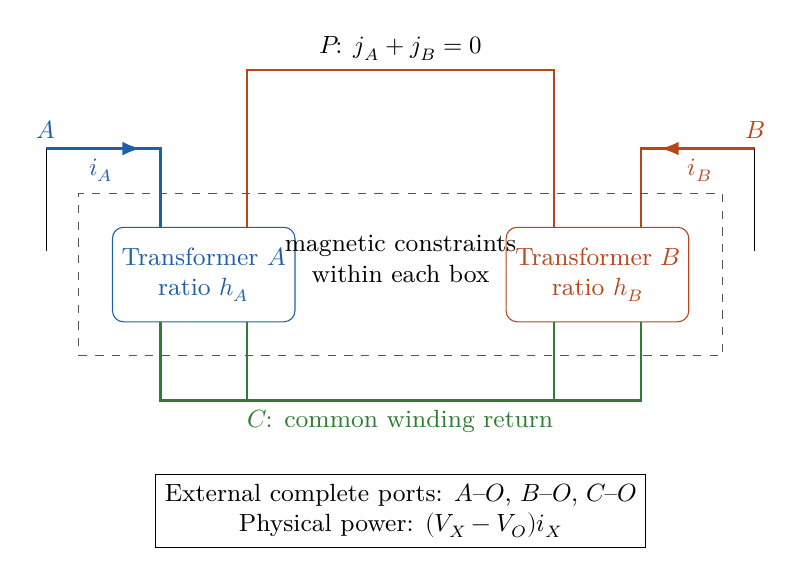
\begin{tikzpicture}[font=\small,>=Latex,
 box/.style={draw,rounded corners,minimum width=2.1cm,minimum height=1.2cm,align=center}]
\node[box,elemA] (ta) at (0,0) {Transformer $A$\\ratio $h_A$};
\node[box,elemB] (tb) at (5,0) {Transformer $B$\\ratio $h_B$};
\draw[elemA,thick] (-2,1.6) node[above] {$A$}--(-.55,1.6)--(-.55,.6);
\draw[elemB,thick] (7,1.6) node[above] {$B$}--(5.55,1.6)--(5.55,.6);
\draw[elemB,thick] (.55,.6)--(.55,2.6)--(4.45,2.6)--(4.45,.6);
\node[above] at (2.5,2.6) {$P$: $j_A+j_B=0$};
\draw[elemC,thick] (-.55,-.6)--(-.55,-1.6)--(5.55,-1.6)--(5.55,-.6);
\draw[elemC,thick] (.55,-.6)--(.55,-1.6) (4.45,-.6)--(4.45,-1.6);
\node[elemC,below] at (2.5,-1.6) {$C$: common winding return};
\draw (-2,1.6)--(-2,.3) (7,1.6)--(7,.3);
\draw[->,elemA,thick] (-1.8,1.6)--(-.8,1.6) node[midway,below] {$i_A$};
\draw[->,elemB,thick] (6.8,1.6)--(5.8,1.6) node[midway,below] {$i_B$};
\node[draw,align=center] (ext) at (2.5,-3) {External complete ports: $A$--$O$, $B$--$O$, $C$--$O$\\
Physical power: $(V_X-V_O)i_X$};
\node[draw,dashed,frameline,fit=(ta)(tb),inner sep=12pt] {};
\node[align=center] at (2.5,.2) {magnetic constraints\\within each box};
\end{tikzpicture}
\end{document}
